{\textbf{1. 平衡二叉树的概念}}

{平衡二叉树(AVL树)是一种特殊的二叉排序树。{其左右子树都是平衡二叉树,且左右子树高度之差的绝对值不超过1}。也可以表述为:以树中所有结点为根的树的左右子树高度之差的绝对值(平衡因子)不超过1。}

{\textbf{2. 平衡二叉树的插入}}

{前面跟二叉排序树的插入一样,就是在插入新的关键字后要进行检查,看新关键字的插入是否会使原平衡二叉树失去平衡,若失去平衡,就要进行平衡调整。}

{当失去平衡的最小子树被调整为平衡子树的时候,原有其他所有不平衡子树无需调整,整个二叉排序树就会成为一棵平衡二叉树。}

失去平衡的最小子树就是以距离插入结点最近,且平衡因子等于2或-2的结点作为根的子树。平衡调整有4种情况,分别为LL型、RR型、LR型和RL型。举例如下,以关键字序列\{16,3,7,11,9,26,18\}构造一棵平衡二叉树,如下图所示。

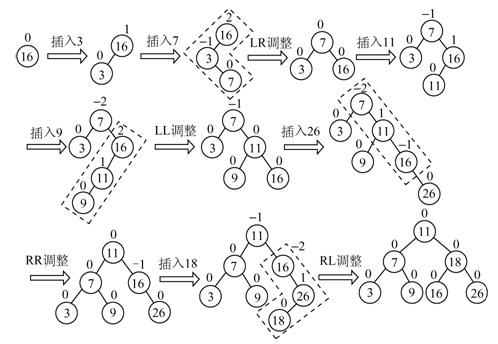
\includegraphics[width=3.70833in,height=2.56250in]{png-jpeg-pics/38C3C4968C61359952421C25368E97F4.png}

{\textbf{3. 平衡二叉树的删除}}

{前面与二叉排序树的删除一样,就是在删除关键字后要进行检查,看新关键字的插入是否会使原平衡二叉树失去平衡,若失去平衡,就要进行平衡调整。}
